\documentclass[10pt]{article}

\usepackage[T1]{fontenc}
\usepackage{geometry}
\usepackage{amsmath, amssymb, amsthm}
\usepackage{graphicx}

\title{Geophysics - Assignment I}
\author{Satvik Saha}
\date{}

\geometry{a4paper, margin=1in}
% \setlength\parindent{0pt}
\renewcommand{\labelenumi}{(\alph{enumi})}
\renewcommand{\labelenumii}{(\roman{enumii})}

\begin{document}
    \noindent\textbf{IISER Kolkata} \hfill \textbf{Assignment I}
    \vspace{3pt}
    \hrule
    \vspace{3pt}
    \begin{center}
        \LARGE{\textbf{ES 2201 : Geophysics}}
    \end{center}
    \vspace{3pt}
    \hrule
    \vspace{3pt}
    Satvik Saha, \texttt{19MS154}\hfill\today
    \vspace{20pt}

    \paragraph{Solution 1.1.} A schematic of the path followed by $P$ waves
    through the earth's interior is presented below.
    \begin{center}
        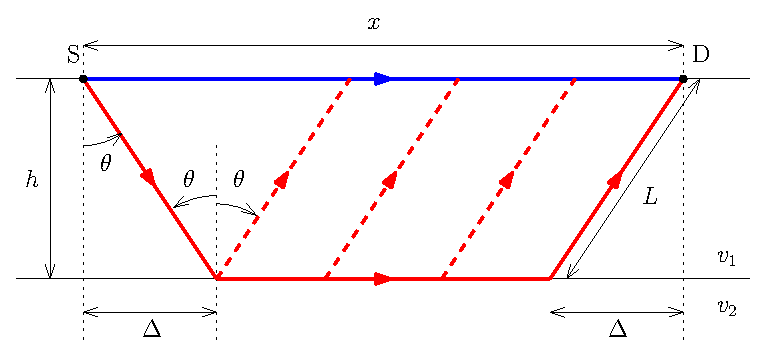
\includegraphics[width=0.7\textwidth]{./seismic_refraction.eps}
    \end{center}
    Note that we have assumed that the waves travel through two layers, both of
    which are isotropic and homogeneous, with the boundaries perfectly horizontal.
    The upper layer has a uniform thickness of $h$.  The wave velocities in the
    upper and lower layers are assumed to be $v_1$ and $v_2$ respectively, with $v_2
    > v_1$. The blue line denotes the path of the $P$ wave which travels from the
    source $S$ (which is assumed to be on the surface) directly to the destination
    $D$ located at a distance $x$ away. The red line shows the path of the wave
    which strikes the interface of the layers at an angle $\theta$, which turns out
    to be the critical angle for reflection so that it continues travelling
    horizontally in the \textit{lower} layer. These wavefronts on the interface emit
    energy upwards in a fashion symmetrical to that of the incidence, so the wave
    which reaches the destination $D$ ascends at the same angle $\theta$.  The
    horizontal component of the distance covered during the descent and ascent of
    the red line is denoted by $\Delta$.

    Let the times taken by the blue and red waves to reach $D$ be $t_1$ and $t_2$
    respectively. Since the blue wave remains in the upper layer throughout, we must
    have $x = v_1t_1$, hence \[
        \boxed{t_1(x) = \frac{x}{v_1}.} 
    \]
    This is the equation of a straight line passing through the origin, with slope
    $1 /v_1$.

    For the red wave, we apply Snell's Law to calculate the angle of incidence for
    which the refracted wave travels horizontally. \[
        \frac{\sin\theta}{v_1} = \frac{\sin(\pi /2)}{v_2}, \qquad
        \qquad \sin\theta = \frac{v_1}{v_2}.
    \] 
    Now, we use simple trigonometry to obtain the horizontal segments $\Delta =
    h\tan\theta$ and the lengths of the slanted red segments $L = h / \cos\theta$.
    The red wave thus travels a distance of $2L$ in the upper layer with speed $v_1$
    and a distance $x - 2\Delta$ in the lower layer with speed $v_2$, so \[
        t_2(x) = \frac{x - 2\Delta}{v_2} + \frac{2L}{v_1} 
            = \frac{x}{v_2} - \left[\frac{2h\tan\theta}{v_2} -
                \frac{2h}{v_1\cos\theta}\right].
        \] 
    This is the equation of a straight line with slope $1 / v_2$.  Note that
    $\Delta$ and $L$ are fixed independently of $x$.  We also note that the red
    waves can be observed only when $x \geq 2\Delta$.  We can make further progress
    by noting that if $\sin\theta = v_1 / v_2$, then \[
        \cos\theta = \frac{\sqrt{v_2^2 - v_1^2}}{v_2}, \qquad
        \tan\theta = \frac{v_1}{\sqrt{v_2^2 - v_1^2}}.
    \] Substituting these expressions, we have \[
        t_2(x) = \frac{x}{v_2} - \left[\frac{2hv_1}{v_2\sqrt{v_2^2 - v_1^2}}
        - \frac{2hv_2}{v_1\sqrt{v_2^2 - v_1^2}}\right]
            = \frac{x}{v_2} - \frac{2h}{\sqrt{v_2^2 - v_1^2}}\left[
            \frac{v_1}{v_2} - \frac{v_2}{v_1}\right].
    \] Simplifying, \[
        \boxed{t_2(x) = \frac{x}{v_2} + \frac{2h}{v_1v_2}\sqrt{v_2^2 -
        v_1^2}.}
    \] 

    Note that since $v_2 > v_1$, the slope of the $t-x$ curve of the blue line is
    \textit{more} than that of the red line. On the other hand, the red line has a
    positive time intercept $t_2(x = 0)$. This means that with increasing $x$, the
    blue wave arrives first until a crossover point where the red wave takes over
    (due to faster travel with $v_2$). This crossover point $x_c$ can be obtained by
    setting $t_1 = t_2$, so \[
        \frac{x_c}{v_1} = \frac{x_c}{v_2} + \frac{2h}{v_1v_2}\sqrt{v_2^2 -
        v_1^2}, \qquad \frac{v_2 - v_1}{v_1v_2}x_c =
        \frac{2h}{v_1v_2}\sqrt{v_2^2 - v_1^2}.
    \] This gives \[
        x_c = 2h\frac{\sqrt{v_2^2 - v_1^2}}{v_2 - v_1} 
                = 2h \sqrt{\frac{v_2 + v_1}{v_2 - v_1}}.
    \] The time of crossover is \[
        t_1(x_c) = t_2(x_c) = 
                \frac{2h}{v_1}\sqrt{\frac{v_2 + v_1}{v_2 - v_1}}.
    \] 
    \begin{center}
        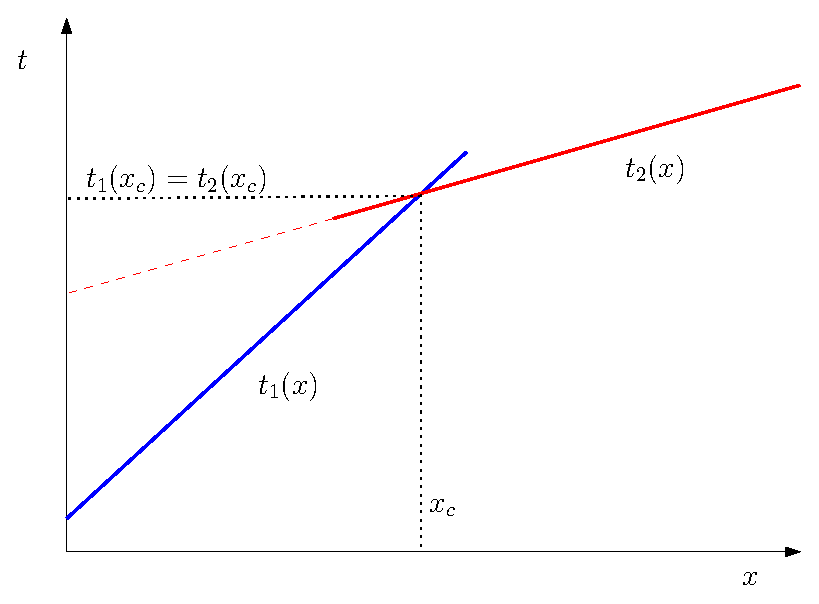
\includegraphics[width=0.6\textwidth]{./T_X.eps}
    \end{center}
    The blue waves are called $P_g$ waves, while the red waves are called $P_n$
    waves. \\

    \textsc{Note}: The blue curve observed in reality does not pass through the
    origin, instead there is a time lag even at $x = 0$, directly above the focus of
    the earthquake.  This is because the focus is typically located at some depth,
    so the waves take some time to reach the surface. If we had to take this into
    account in our analysis, the blue curve would not be linear. Supposing the depth
    of the focus to be $f$, we see that the distance to the receiving station is
    $\sqrt{f^2 + x^2}$, so the arrival time is given by \[
        t_1'(x) = \frac{\sqrt{f^2 + x^2}}{v_1}.
    \] When $f /x$ is small, we can write $\sqrt{1 + f^2/x^2} \approx 1 + f^2
    /2x^2$, so \[
        t_1'(x) \approx \frac{x}{v_1} + \frac{f^2}{2v_1x}.
    \] As $x$ grows large, we get back our simpler expression $t_1'(x) \to x / v_1$.

    \paragraph{Solution 1.2}
    \begin{enumerate}
        \item \begin{enumerate}
            \item The $S$ wave velocity curve vanishes in the outer core region, and
            reappears in the inner core.
            \item The $P$ and $S$ wave velocities seem to increase with depth along 
            with density, except at points of discontinuity where they jump up or
            down.
            The major drop in $P$ wave velocity is at the $D''$ layer as they enter
            the outer core.
            \item The density profile has a major jump upwards, also at the $D''$
            layer marking the outer core.
            \item Both $P$ and $S$ wave velocities rise greatly after exiting the
            crust, before suffering a dip in the LVZ (Low Velocity Zone).
            The $S$ wave velocity drop is slightly more pronounced.
            The density curve shows a similar trend in this region.
            These changes are comparitively smooth.
            \item The $P$ wave velocities are always higher than $S$ wave velocities
            in a given zone.
        \end{enumerate}

        \item \begin{enumerate}
            \item The fact that the $S$ waves vanish in the outer core indicates 
            a liquid outer core. 
            The reappearance of $S$ waves in the inner core suggests that it is
            solid.
            \item The smooth changes (increase) in $P$ and $S$ wave velocity
            indicate that the material in those regions is largely the same.
            The points of discontinuity mark regions where the material changes
            abruptly, in terms of physical properties.
            \item The major jump in density at the outer core indicates a change in
            composition of the material, and reinforces the idea of a change in
            state.
            \item The LVZ is not compositionally too different from the surrounding
            zones; instead, this zone may have liquid components.  It is not
            completely liquid, but rather is partially melted.
            \item The $P$ wave velocity depends on some additional terms compared to
            the $S$ waves, which is natural since their physical natures differ
            (compression waves vs shear waves). The $P$ wave velocity is not merely
            a scaled up form of the $S$ wave velocity.
        \end{enumerate}

        \item \begin{enumerate}
            \item $S$ waves are shear waves, which can only properly travel in
            solids where a restoring force acts on material moved perpendicular to
            the propagation of the wave. Thus, a liquid outer core would explain why
            $S$ waves aren't present there.
            
            The presence of $S$ waves in the inner core thus suggests that it is
            solid. These waves cannot be the same waves generated from the surface,
            nor from outside the outer core which acts as a barrier. Thus, these
            must be generated either within the inner core or from the inner-outer
            core interface, where there may be moving liquid material.

            \item In a zone where the wave velocities and density vary smoothly
            (such as in the bulk of the lower mantle or within the outer core), any
            abrupt changes in material composition would be reflected as an abrupt
            velocity change. The smooth density increase with depth follows
            naturally due to the weight of the layers above.

            The wave velocities depend on this density too, as \[
                v_P = \sqrt{\frac{\kappa + 4\mu /3}{\rho}}, \qquad
                v_S = \sqrt{\frac{\mu}{\rho}},
            \] where $\kappa$ is the bulk modulus of the material, $\mu$ is the
            shear modulus, and $\rho$ is the density.
            This would seem to indicate that wave velocity and density ought to have
            opposing trends -- however, the shear modulus $\mu$ and bulk modulus
            $\kappa$ also increase with depth and have a density dependence, which
            outweighs the denominator.

            The wave velocities can be seen to vary smoothly with physical
            properties -- thus, discontinuities in velocity mark discontinuities in
            these physical properties.

            \item Such a large jump at the $D''$ layer is unlikely to arise purely
            from a change in composition, where gradual movement of material would
            perhaps smooth things out. The high density indicates the presence of
            metal such as iron.

            \item Again, a smooth velocity and density change indicates a gradual
            change in the physical properties of the material in that zone.
            The fact that the $S$ wave velocity drops more than the $P$ wave
            velocity indicates the presence of some amount of liquid.
            A complete liquid state would obstruct the passage of $S$ waves in that
            region. Instead, a partially melted zone would explain the velocity
            drops.

            \item The fact that the $P$ waves are faster than $S$ waves is evident
            from their velocity formulae, which we can rearrange as \[
                v_P^2 - v_S^2 = \frac{\kappa + \mu /3}{\rho} > 0.
            \]
        \end{enumerate}
    \end{enumerate}

\end{document}
